% Provenance (never printed): see sources/outline_sources.md (Year 1:
% geological cross-sections, apparent dip, thickness, boreholes). Every
% Varden Hills number comes from figdata/bachelor-1/varden_sections.py, which
% imports the shared model figdata/shared/region.py; numbers of the exercises
% and problem in the Book 3 scratch calculator and in that script's values.
\chapter{Cortes geológicos}\label{ch:b1:cross-sections}

Una empresa de ingeniería planea un túnel bajo las colinas de Varden, recto de oeste a este, a una
altitud constante de \qty{200}{m}. Antes de perforar un solo metro, los geólogos deben decir qué
rocas cortará la máquina, dónde cruzará la falla y cuánto tiempo pasará en la caliza, una roca que
puede contener cavidades abiertas y agua. Nadie puede ver dentro de las colinas; pero el \omterm{def:b1:geological-maps:geological-map}{mapa
geológico} de \cref{ch:b1:geological-maps}, unos pocos sondeos y la geometría de los planos bastan
para dibujar una rebanada vertical del terreno ---un corte geológico--- y leer en ella las
respuestas. Este capítulo enseña cómo se construye un corte a partir de un mapa, cómo cambian los
\omterm{def:b1:geological-maps:attitude}{buzamientos} y los espesores cuando la rebanada se corta oblicuamente, cómo se correlacionan los
sondeos y cómo un corte cuenta la historia de las rocas que atraviesa. Termina con el túnel.

\begin{recall}
La \omterm{def:b1:geological-maps:attitude}{actitud} de un plano viene dada por su \omterm{def:b1:geological-maps:attitude}{dirección de buzamiento} $\alpha$ y su \omterm{def:b1:geological-maps:attitude}{buzamiento}
$\delta$, y el plano que pasa por un punto de altitud $z_0$ en el origen es
$z = z_0 - \tan\delta\,(x\sin\alpha + y\cos\alpha)$; tres puntos de un contacto fijan su \omterm{def:b1:geological-maps:attitude}{actitud};
la regla de la V permite leer el \omterm{def:b1:geological-maps:attitude}{buzamiento} a partir del patrón de afloramiento en los valles
(\cref{ch:b1:geological-maps}). Una curva de nivel une, en un mapa topográfico, puntos de igual
altitud (libro 1, año 9). Las rocas más jóvenes se apoyan sobre las más antiguas, y lo que corta a
una roca es más joven que ella (libro 1, año 7).
\end{recall}

\section{Del mapa al corte}

\begin{definition}[Corte geológico, perfil topográfico, exageración vertical]\label{def:b1:cross-sections:section}
Un \emph{corte geológico}\index{corte geológico} es un dibujo de las unidades de roca y de las
estructuras en un plano vertical a través del terreno, a lo largo de una línea trazada en el mapa.
Su borde superior es el \emph{perfil topográfico}\index{perfil topográfico}, la curva de la altitud
del terreno a lo largo de la línea. La \emph{exageración vertical}\index{exageración vertical} $e$
de un corte es el cociente entre su escala vertical y su escala horizontal; un corte es
\emph{a escala verdadera} cuando $e = 1$.
\end{definition}

\begin{method}[Construcción de un corte geológico a partir de un mapa]\label{met:b1:cross-sections:construct}
\begin{enumerate}
  \item Trácese la línea del corte en el mapa y apóyese a lo largo de ella el borde de una tira de
        papel; márquense los puntos donde cada curva de nivel la cruza, con su altitud, y donde la
        cruza cada contacto y cada falla.
  \item Trácese una línea base horizontal de la misma longitud y una escala vertical de altitudes
        (elíjase $e$ y escríbase en el corte).
  \item Llévese cada marca de curva de nivel a su altitud y únanse los puntos suavemente: este es el
        \omterm{def:b1:cross-sections:section}{perfil topográfico}.
  \item Llévese cada contacto y cada falla al perfil, en el punto donde cruzan la línea.
  \item Desde cada uno de esos puntos, trácese el contacto hacia el interior del terreno con su
        \omterm{def:b1:geological-maps:attitude}{buzamiento} \emph{en el plano del corte} ---su \omterm{def:b1:cross-sections:apparent-dip}{buzamiento aparente}
        (\cref{sec:b1:cross-sections:apparent})--- exagerado por $e$ si $e \ne 1$; úsense los
        sondeos y las curvas de nivel de la estructura donde los haya.
  \item Complétense las unidades entre los \omterm{def:b1:geological-maps:geological-map}{contactos}, respetando el orden de superposición y los
        cortes, y añádanse la leyenda, las escalas, la orientación de la línea y $e$.
\end{enumerate}
\end{method}

\begin{omfigure}
\begin{tikzpicture}[font=\scriptsize, x=1cm, y=1cm]
% map strip with contours crossing the section line
\draw[black!50] (0,2.7) rectangle (9,4.5);
\foreach \x/\h in {0.7/300, 1.6/350, 2.6/400, 4.1/400, 5.0/350, 5.8/300, 7.2/300, 8.2/350} {
  \draw[contour, brown!70!black] (\x-0.25,2.7) .. controls (\x+0.1,3.4) and (\x-0.1,3.8) .. (\x+0.2,4.5);
  \node[brown!60!black, above] at (\x+0.2,4.5) {\h};
}
\draw[omThm, thick] (0,3.6) node[left] {X} -- (9,3.6) node[right] {Y};
\fill[omDef] (3.4,3.6) circle (1.5pt);
\node[omDef, fill=white, inner sep=1pt, above right] at (3.4,3.62) {contacto};
% profile
\draw[->] (0,-0.1) -- (0,1.95) node[above] {altitud (m)};
\draw (0,0) -- (9,0);
\foreach \y/\l in {0/250, 0.5/300, 1.0/350, 1.5/400} { \draw (-0.08,\y) -- (0,\y); \node[left] at (-0.08,\y) {\l}; }
\coordinate (p1) at (0.85,0.5); \coordinate (p2) at (1.75,1.0); \coordinate (p3) at (2.75,1.5);
\coordinate (p4) at (4.25,1.5); \coordinate (p5) at (5.15,1.0); \coordinate (p6) at (5.95,0.5);
\coordinate (p7) at (7.35,0.5); \coordinate (p8) at (8.35,1.0);
\foreach \i/\x in {1/0.85,2/1.75,3/2.75,4/4.25,5/5.15,6/5.95,7/7.35,8/8.35} {
  \draw[black!35, densely dotted] (\x,3.6) -- (p\i);
  \fill (p\i) circle (1.2pt);
}
\draw[thick] (0,0.2) .. controls (0.5,0.3) .. (p1) .. controls (1.3,0.8) .. (p2) .. controls (2.3,1.35) .. (p3)
  .. controls (3.5,1.85) .. (p4) .. controls (4.7,1.25) .. (p5) .. controls (5.5,0.7) .. (p6)
  .. controls (6.6,0.25) .. (p7) .. controls (7.9,0.75) .. (p8) .. controls (8.7,1.15) .. (9,1.2);
\draw[omDef, densely dotted] (3.4,3.6) -- (3.4,1.72);
\draw[omDef, thick] (3.4,1.72) -- (4.45,0.05);
\node[omDef, below right] at (4.3,-0.02) {contacto, trazado con su buzamiento aparente};
\end{tikzpicture}

{\small Construcción de un corte (esquema): los cruces de las curvas de nivel con la línea X--Y se
llevan hacia abajo a sus altitudes para dar el \omterm{def:b1:cross-sections:section}{perfil topográfico}; un contacto que cruza la línea
se lleva al perfil y se dibuja en el terreno con su \omterm{def:b1:cross-sections:apparent-dip}{buzamiento aparente}.}
\end{omfigure}

La sección siguiente se construyó por ordenador a partir del modelo de las colinas de Varden a lo
largo de la línea C--D, que va exactamente hacia el este a través del mapa en $y = \qty{6}{km}$.
Muestra el \omterm{def:b1:geological-maps:fold}{anticlinal} cuyo núcleo de arenisca y basamento aparece en $x \approx \qty{3.5}{km}$, la
caliza y la lutita en sus flancos, la creta en el \omterm{def:b1:geological-maps:fold}{sinclinal} al este y la falla normal. La línea del
túnel, a \qty{200}{m}, y los sondeos B1, B2, B3 de \cref{sec:b1:cross-sections:boreholes} se dibujan
sobre ella.

\begin{omfigure}
\begin{tikzpicture}
\begin{axis}[x=1.4cm, y=0.0042cm, xmin=0, xmax=10, ymin=-500, ymax=650,
  axis on top, tick label style={font=\scriptsize}, label style={font=\small},
  xlabel={distancia hacia el este desde C (km)}, ylabel={altitud (m)},
  ytick={-400,-200,0,200,400,600}, clip=true]
\addplot[lith schist, draw=black, line width=0.3pt, even odd rule] table {figdata/out/bachelor-1-varden_sections-cd-unit-schist.dat};
\addplot[lith granite, draw=black, line width=0.3pt, even odd rule] table {figdata/out/bachelor-1-varden_sections-cd-unit-granite.dat};
\addplot[om lith={icsTriassic!35}{om sand}, draw=black, line width=0.3pt, even odd rule] table {figdata/out/bachelor-1-varden_sections-cd-unit-sandstone.dat};
\addplot[om lith={icsJurassic!40}{om limestone}, draw=black, line width=0.3pt, even odd rule] table {figdata/out/bachelor-1-varden_sections-cd-unit-limestone.dat};
\addplot[om lith={icsJurassic!15}{om shale}, draw=black, line width=0.3pt, even odd rule] table {figdata/out/bachelor-1-varden_sections-cd-unit-shale.dat};
\addplot[om lith={icsCretaceous!35}{om limestone}, draw=black, line width=0.3pt, even odd rule] table {figdata/out/bachelor-1-varden_sections-cd-unit-chalk.dat};
\addplot[lith alluvium, draw=black, line width=0.3pt, even odd rule] table {figdata/out/bachelor-1-varden_sections-cd-unit-alluvium.dat};
\addplot[black, line width=0.8pt] table {figdata/out/bachelor-1-varden_sections-cd-ground.dat};
\addplot[fault, line width=1.1pt] table {figdata/out/bachelor-1-varden_sections-cd-fault.dat};
\addplot[omThm, line width=1.4pt] coordinates {(1,200) (9,200)};
\node[omThm, font=\scriptsize, fill=white, inner sep=1pt, below] at (axis cs:8.3,190) {túnel, \qty{200}{m}};
\draw[blue!60!black, line width=0.9pt] (axis cs:1.5,-480) -- (axis cs:1.5,524);
\draw[blue!60!black, line width=0.9pt] (axis cs:3.5,-480) -- (axis cs:3.5,381);
\draw[blue!60!black, line width=0.9pt] (axis cs:5.5,-480) -- (axis cs:5.5,530);
\node[font=\scriptsize, blue!60!black, fill=white, inner sep=1pt] at (axis cs:1.5,-440) {B1};
\node[font=\scriptsize, blue!60!black, fill=white, inner sep=1pt] at (axis cs:3.5,-440) {B2};
\node[font=\scriptsize, blue!60!black, fill=white, inner sep=1pt] at (axis cs:5.5,-440) {B3};
\node[font=\small, above right] at (axis cs:0,650) {C (oeste)};
\node[font=\small, above left] at (axis cs:10,650) {D (este)};
\end{axis}
\end{tikzpicture}

\smallskip
\begin{tikzpicture}
\begin{axis}[x=1.4cm, y=0.0014cm, xmin=0, xmax=10, ymin=-500, ymax=650,
  axis on top, tick label style={font=\scriptsize}, ytick={-500,0,500},
  xticklabels={}, clip=true]
\addplot[lith schist, draw=black, line width=0.2pt, even odd rule] table {figdata/out/bachelor-1-varden_sections-cd-unit-schist.dat};
\addplot[lith granite, draw=black, line width=0.2pt, even odd rule] table {figdata/out/bachelor-1-varden_sections-cd-unit-granite.dat};
\addplot[om lith={icsTriassic!35}{om sand}, draw=black, line width=0.2pt, even odd rule] table {figdata/out/bachelor-1-varden_sections-cd-unit-sandstone.dat};
\addplot[om lith={icsJurassic!40}{om limestone}, draw=black, line width=0.2pt, even odd rule] table {figdata/out/bachelor-1-varden_sections-cd-unit-limestone.dat};
\addplot[om lith={icsJurassic!15}{om shale}, draw=black, line width=0.2pt, even odd rule] table {figdata/out/bachelor-1-varden_sections-cd-unit-shale.dat};
\addplot[om lith={icsCretaceous!35}{om limestone}, draw=black, line width=0.2pt, even odd rule] table {figdata/out/bachelor-1-varden_sections-cd-unit-chalk.dat};
\addplot[lith alluvium, draw=black, line width=0.2pt, even odd rule] table {figdata/out/bachelor-1-varden_sections-cd-unit-alluvium.dat};
\addplot[black, line width=0.6pt] table {figdata/out/bachelor-1-varden_sections-cd-ground.dat};
\addplot[fault, line width=0.8pt] table {figdata/out/bachelor-1-varden_sections-cd-fault.dat};
\end{axis}
\end{tikzpicture}

{\small Corte C--D a través de las colinas de Varden, a partir del modelo de la región. Arriba:
\omterm{def:b1:cross-sections:section}{exageración vertical} $e = 3$; abajo: el mismo corte a escala verdadera ($e = 1$), donde los flancos
de \ang{12} parecen tan suaves como son. Colores como en el \omterm{def:b1:geological-maps:geological-map}{mapa geológico} de
\cref{ch:b1:geological-maps}; la falla (línea gruesa) es la falla normal, cuyo bloque oriental está
hundido. La línea roja es el túnel del problema; B1--B3 son sondeos.}
\end{omfigure}

La \omterm{def:b1:cross-sections:section}{exageración vertical} hace legibles las unidades delgadas y el relieve suave, pero deforma todos
los ángulos: los flancos de \ang{12} del \omterm{def:b1:geological-maps:fold}{pliegue} aparecen en torno a \ang{32} en el corte superior.
La sección siguiente dice exactamente cómo.

\section{Buzamiento aparente}\label{sec:b1:cross-sections:apparent}

\begin{definition}[Buzamiento aparente]\label{def:b1:cross-sections:apparent-dip}
El \emph{buzamiento aparente}\index{buzamiento aparente} $\beta$ de un plano en un corte vertical
dado es el ángulo entre la horizontal y la traza del plano en ese corte. Es igual al \omterm{def:b1:geological-maps:attitude}{buzamiento}
verdadero $\delta$ cuando el corte sigue la \omterm{def:b1:geological-maps:attitude}{dirección de buzamiento}, y es cero cuando sigue el \omterm{def:b1:geological-maps:attitude}{rumbo}.
\end{definition}

\begin{theorem}[Cálculo del buzamiento aparente]\label{thm:b1:cross-sections:apparent-dip}
Un plano de \omterm{def:b1:geological-maps:attitude}{buzamiento} $\delta$ y \omterm{def:b1:geological-maps:attitude}{dirección de buzamiento} $\alpha$, cortado por un corte vertical
de \omterm{def:b1:spherical-astronomy:horizontal}{acimut} $\theta$, muestra el \omterm{def:b1:cross-sections:apparent-dip}{buzamiento aparente} $\beta$ con
\[
  \tan\beta = \tan\delta\,\cos\gamma, \qquad \gamma = \alpha - \theta ,
\]
el plano desciende en la dirección $\theta$ cuando $\cos\gamma > 0$. En particular $|\beta| \le \delta$, con igualdad solo en la \omterm{def:b1:geological-maps:attitude}{dirección de buzamiento}.
\end{theorem}

\begin{proof}
Tómese el plano $z = z_0 - \tan\delta\,(x\sin\alpha + y\cos\alpha)$ de
\cref{ch:b1:geological-maps}. A lo largo del corte, un paso horizontal de longitud $s$ en la
dirección $\theta$ es $(x, y) = s(\sin\theta, \cos\theta)$, así que $z = z_0 - s\tan\delta\,(\sin\theta\sin\alpha + \cos\theta\cos\alpha) =
z_0 - s\tan\delta\cos(\alpha - \theta)$. La traza es una recta que desciende $\tan\delta\cos\gamma$
por unidad de distancia horizontal: es decir, $\tan\beta$. Como $|\cos\gamma| \le 1$,
$|\tan\beta| \le \tan\delta$.
\end{proof}

\begin{omfigure}
\begin{tikzpicture}[font=\scriptsize, x={(1cm,0cm)}, y={(0.6cm,0.45cm)}, z={(0cm,1cm)}]
% hidden edges of the block
\draw[black!30, densely dashed] (0,0,0) -- (0,3,0) -- (4,3,0);
\draw[black!30, densely dashed] (0,3,0) -- (0,3,2);
% the oblique vertical section, from the front-left corner to the back-right one
\fill[black!10, opacity=0.7] (0,0,0) -- (4,3,0) -- (4,3,2) -- (0,0,2) -- cycle;
\draw[black!45] (0,0,0) -- (4,3,0) -- (4,3,2);
% the dipping plane, from the top-west edge down to the base
\fill[omDef!25, opacity=0.75] (0,0,2) -- (2.6,0,0) -- (2.6,3,0) -- (0,3,2) -- cycle;
\draw[omDef] (2.6,0,0) -- (2.6,3,0);
\draw[omDef, very thick] (0,0,2) -- (2.6,0,0);
\draw[omThm, very thick] (0,0,2) -- (2.6,1.95,0);
% visible edges of the block
\draw[black!70] (0,0,0) -- (4,0,0) -- (4,0,2) -- (0,0,2) -- cycle;
\draw[black!70] (0,0,2) -- (0,3,2) -- (4,3,2) -- (4,0,2);
\draw[black!70] (4,0,0) -- (4,3,0) -- (4,3,2);
% labels
\draw[omDef] (2.0,0,0) arc[start angle=180, end angle=142.4, radius=0.6cm];
\node[omDef] at (1.7,0,0.2) {$\delta$};
\node[omDef, below, align=center] at (1.3,0,0) {cara frontal, en la dirección de buzamiento:\\ buzamiento verdadero $\delta$};
\node[omThm, right, align=left] at (4.45,2.2,0.3) {corte oblicuo (gris):\\ buzamiento aparente $\beta < \delta$};
\node[above] at (0,1.5,2) {N};
\draw[->] (0.15,1.5,2.05) -- (0.15,2.2,2.05);
\end{tikzpicture}

{\small \omterm{def:b1:cross-sections:apparent-dip}{Buzamiento aparente} (bloque esquemático). Un plano que buza hacia el este (azul) muestra su
\omterm{def:b1:geological-maps:attitude}{buzamiento} verdadero $\delta$ en la cara frontal, una cara vertical cortada en la \omterm{def:b1:geological-maps:attitude}{dirección de
buzamiento}; en el corte vertical gris, cortado oblicuamente, su traza (roja) desciende más
suavemente, con el \omterm{def:b1:cross-sections:apparent-dip}{buzamiento aparente} $\beta$; en un corte a lo largo del \omterm{def:b1:geological-maps:attitude}{rumbo}, norte--sur,
sería horizontal.}
\end{omfigure}

\begin{proposition}[Ángulos en un corte exagerado]\label{prop:b1:cross-sections:exaggeration}
En un corte dibujado con \omterm{def:b1:cross-sections:section}{exageración vertical} $e$, una recta de \omterm{def:b1:cross-sections:apparent-dip}{buzamiento aparente} $\beta$ se
dibuja con el ángulo $\beta'$, con $\tan\beta' = e\tan\beta$.
\end{proposition}

\begin{proof}
Sobre una distancia horizontal $s$ la recta desciende $s\tan\beta$; dibujada con una escala
vertical $e$ veces la horizontal, la caída aparece como $es\tan\beta$ sobre la misma longitud
dibujada $s$.
\end{proof}

\begin{example}
El flanco oriental del \omterm{def:b1:geological-maps:fold}{anticlinal} de Varden buza \ang{12.16} hacia \ang{080.7}
(\cref{ch:b1:geological-maps}). En el corte oeste--este C--D,
$\gamma = \ang{80.7} - \ang{90} = \ang{-9.3}$, y $\tan\beta =
\tan\ang{12.16}\cos\ang{9.3} = 0.2154\times0.9868 = 0.2126$: $\beta =
\ang{12.0}$. Dibujado con $e = 3$, aparece en $\arctan(3\times0.2126) =
\ang{32.5}$. En el corte A--B de \omterm{def:b1:spherical-astronomy:horizontal}{acimut} \ang{071.6}, $\gamma = \ang{9.1}$
y $\beta = \ang{12.0}$ también: ambos cortes siguen de cerca la \omterm{def:b1:geological-maps:attitude}{dirección de buzamiento}. La falla,
que buza \ang{60} hacia \ang{120}, tiene en C--D el \omterm{def:b1:cross-sections:apparent-dip}{buzamiento aparente} $\arctan(\tan\ang{60}\cos\ang{30}) = \arctan 1.5 = \ang{56.3}$.
\end{example}

\section{Espesor}

\begin{definition}[Espesor verdadero, espesor vertical]\label{def:b1:cross-sections:thickness}
El \emph{espesor verdadero}\index{espesor verdadero} $t$ de una capa es la distancia entre su base y su techo medida
perpendicularmente a la estratificación. Su \emph{espesor vertical}\index{espesor vertical} $h$ es la misma distancia
medida a lo largo de la vertical, tal como la corta un sondeo vertical.
\end{definition}

\begin{proposition}[Espesor de una capa buzante]\label{prop:b1:cross-sections:thickness}
Para una capa de \omterm{def:b1:geological-maps:attitude}{buzamiento} $\delta$:
\begin{enumerate}
  \item $t = h\cos\delta$;
  \item sobre terreno horizontal, si el afloramiento de la capa tiene la anchura $w$ medida perpendicularmente al \omterm{def:b1:geological-maps:attitude}{rumbo},
        $t = w\sin\delta$;
  \item sobre un terreno con pendiente $\sigma$ en la dirección perpendicular al \omterm{def:b1:geological-maps:attitude}{rumbo}, con $w$ medida a lo largo del terreno,
        $t = w\sin(\delta + \sigma)$ si el terreno desciende en sentido contrario al \omterm{def:b1:geological-maps:attitude}{buzamiento}, y
        $t = w\sin(\delta - \sigma)$ si desciende en el mismo sentido, pero menos inclinado que los estratos.
\end{enumerate}
\end{proposition}

\begin{proof}
En el plano vertical perpendicular al \omterm{def:b1:geological-maps:attitude}{rumbo}, la base y el techo de la capa son dos rectas paralelas inclinadas $\delta$,
separadas una distancia $t$. (1) Un segmento vertical que las une forma con su normal común el ángulo $\delta$, así que
$t = h\cos\delta$. (2)--(3) Un segmento de longitud $w$ que las une a lo largo del terreno forma con la estratificación el
ángulo $\delta$ cuando el terreno es horizontal, $\delta + \sigma$ cuando el terreno sube en sentido contrario al \omterm{def:b1:geological-maps:attitude}{buzamiento}
(las dos inclinaciones se suman), y $\delta - \sigma$ cuando baja en el mismo sentido; la distancia entre las rectas paralelas
es la longitud del segmento por el seno de ese ángulo.
\end{proof}

\begin{omfigure}
\begin{tikzpicture}[font=\scriptsize]
\pgfmathsetmacro{\d}{25}\pgfmathsetmacro{\t}{1.3}
\pgfmathsetmacro{\h}{\t/cos(\d)}\pgfmathsetmacro{\w}{\t/sin(\d)}
\pgfmathsetmacro{\X}{4.0}
\fill[icsJurassic!30] (-\w,0) -- (0,0) -- (\X,{-\X*tan(\d)}) -- (\X,{-\X*tan(\d)-\h}) -- cycle;
\draw[thick] (0,0) -- (\X,{-\X*tan(\d)}) node[right] {techo de la capa};
\draw[thick] (-\w,0) -- (\X,{-\X*tan(\d)-\h}) node[right] {base};
\draw[black!70] ({-\w-0.8},0) -- (\X+0.6,0) node[right] {terreno horizontal};
% vertical thickness
\draw[omThm, thick, <->] (1.0,{-1.0*tan(\d)}) -- (1.0,{-1.0*tan(\d)-\h});
\node[omThm, right] at (1.0,{-1.0*tan(\d)-0.55*\h}) {$h$};
% true thickness, perpendicular to the bedding
\coordinate (A) at (2.8,{-2.8*tan(\d)});
\draw[omDef, thick, <->] (A) -- ++({-90-\d}:\t);
\node[omDef, right] at ($(A)+({-90-\d}:0.5*\t)$) {$t$};
% outcrop width on flat ground
\draw[black, thick, <->] (-\w,0.2) -- (0,0.2);
\node[above] at ({-0.5*\w},0.2) {$w$};
\draw[omThm] (1.0,0) arc[start angle=0, end angle=-\d, radius=1.0];
\node[omThm] at (1.25,-0.22) {$\delta$};
\end{tikzpicture}

{\small Espesores de una capa buzante en el plano vertical perpendicular al \omterm{def:b1:geological-maps:attitude}{rumbo}: el \omterm{def:b1:cross-sections:thickness}{espesor
verdadero} $t$, perpendicular a la estratificación; el \omterm{def:b1:cross-sections:thickness}{espesor vertical} $h = t/\cos\delta$; la
anchura del afloramiento $w = t/\sin\delta$ sobre terreno horizontal (esquema, con $\delta = \ang{25}$).}
\end{omfigure}

En las colinas de Varden, un sondeo que entra en la caliza por arriba la atraviesa a lo largo de \qty{180}{m} de testigo:
ese es su \omterm{def:b1:cross-sections:thickness}{espesor vertical}. Su \omterm{def:b1:cross-sections:thickness}{espesor verdadero} es $180\cos\ang{12.16} = \qty{176.0}{m}$. Una
unidad delgada y una unidad gruesa pueden mostrar la misma anchura de afloramiento si sus
\omterm{def:b1:geological-maps:attitude}{buzamientos} difieren, y una capa empinada puede mostrar un afloramiento ancho en una ladera que
corre con ella: el espesor nunca se lee directamente de un mapa.

\section{Sondeos y curvas de nivel de la estructura}\label{sec:b1:cross-sections:boreholes}

\begin{definition}[Registro de sondeo, correlación]\label{def:b1:cross-sections:log}
Un \emph{registro de sondeo}\index{registro de sondeo} es la anotación, frente a la profundidad, de
las rocas que atraviesa un sondeo: las unidades, las profundidades de sus \omterm{def:b1:geological-maps:geological-map}{contactos} y cualquier
propiedad medida. La \emph{correlación}\index{correlación (de registros)} es el emparejamiento de
las mismas unidades y \omterm{def:b1:geological-maps:geological-map}{contactos} de un registro a otro.
\end{definition}

Tres sondeos perforados en la línea C--D dan las siguientes profundidades bajo el terreno de la base
de cada unidad (un guion: el contacto queda por encima del terreno, erosionado):
\begin{center}
\small
\begin{tabular}{lcccccc}
\hline
sondeo & $x$ (km) & terreno (m) & creta & lutita & caliza & arenisca \\
\hline
B1 & 1.5 & 524.02 & 388.98 & 488.98 & 668.98 & 788.98 \\
B2 & 3.5 & 380.64 & --- & --- & 100.48 & 220.48 \\
B3 & 5.5 & 529.98 & 394.93 & 494.93 & 674.93 & 794.93 \\
\hline
\end{tabular}
\end{center}
B2 empieza en la caliza, en la cresta del \omterm{def:b1:geological-maps:fold}{anticlinal}; B1 y B3 empiezan en la creta, en sus flancos.
Restando las profundidades a la altitud del terreno se obtienen las altitudes de los \omterm{def:b1:geological-maps:geological-map}{contactos}: la
base de la caliza queda en $380.64 - 100.48 = \qty{280.16}{m}$ en B2 y en $529.98 - 674.93 =
\qty{-144.95}{m}$ en B3, \qty{425.11}{m} más abajo a lo largo de \qty{2}{km}, una pendiente de
\num{0.2126}: el \omterm{def:b1:cross-sections:apparent-dip}{buzamiento aparente} de \ang{12.0} hallado antes. B1 y B3 dan los mismos
espesores, \qty{100}{m} de lutita, \qty{180}{m} de caliza y \qty{120}{m} de arenisca: las unidades
tienen el mismo \omterm{def:b1:cross-sections:thickness}{espesor vertical} en ambos flancos.

\begin{omfigure}
\begin{tikzpicture}[font=\scriptsize, x=1cm, y=0.0045cm]
\foreach \b/\xx/\g/\c/\s/\l/\sd in {B1/0/524.02/388.98/488.98/668.98/788.98, B3/6/529.98/394.93/494.93/674.93/794.93} {
  \begin{scope}[xshift=\xx cm]
  \fill[icsCretaceous!35] (0,{\g}) rectangle (0.9,{\g-\c});
  \fill[icsJurassic!15] (0,{\g-\c}) rectangle (0.9,{\g-\s});
  \fill[icsJurassic!40] (0,{\g-\s}) rectangle (0.9,{\g-\l});
  \fill[icsTriassic!35] (0,{\g-\l}) rectangle (0.9,{\g-\sd});
  \fill[black!15] (0,{\g-\sd}) rectangle (0.9,{\g-\sd-40});
  \draw (0,{\g}) rectangle (0.9,{\g-\sd-40});
  \node[above] at (0.45,{\g}) {\b};
  \end{scope}
}
\begin{scope}[xshift=3cm]
  \fill[icsJurassic!40] (0,380.64) rectangle (0.9,280.16);
  \fill[icsTriassic!35] (0,280.16) rectangle (0.9,160.16);
  \fill[black!15] (0,160.16) rectangle (0.9,120);
  \draw (0,380.64) rectangle (0.9,120);
  \node[above] at (0.45,380.64) {B2};
\end{scope}
% correlation lines: base of limestone
\draw[omThm, dashed] (0.9,-144.96) -- (3,280.16);
\draw[omThm, dashed] (3.9,280.16) -- (6,-144.95);
\draw[omDef, dashed] (0.9,-264.96) -- (3,160.16);
\draw[omDef, dashed] (3.9,160.16) -- (6,-264.95);
% elevation axis
\draw[->] (-0.6,-320) -- (-0.6,600) node[above] {altitud (m)};
\foreach \y in {-200,0,200,400} { \draw (-0.68,\y) -- (-0.6,\y); \node[left] at (-0.68,\y) {\y}; }
\foreach \c/\yy/\n in {icsCretaceous!35/400/creta, icsJurassic!15/340/lutita, icsJurassic!40/280/caliza, icsTriassic!35/220/arenisca, black!15/160/basamento} {
  \fill[\c] (7.2,\yy) rectangle (7.45,\yy+36); \draw (7.2,\yy) rectangle (7.45,\yy+36);
  \node[right] at (7.45,\yy+18) {\n};
}
\node[omThm, right] at (0.95,480) {base de la caliza};
\node[omDef, left] at (4.0,-250) {base de la arenisca};
\end{tikzpicture}

{\small Los registros de los sondeos B1, B2 y B3 sobre la línea C--D, colgados a sus altitudes
verdaderas (no a escala horizontal), y su \omterm{def:b1:cross-sections:log}{correlación}: la base de la caliza (roja) y la de la
arenisca (azul) suben desde ambos flancos hasta la cresta del \omterm{def:b1:geological-maps:fold}{anticlinal} en B2.}
\end{omfigure}

Donde hay muchos sondeos, la forma de un contacto enterrado se cartografía con \omterm{def:b1:cross-sections:structure-contour}{curvas de nivel
estructurales}.

\begin{definition}[Curva de nivel estructural, mapa de curvas de nivel estructurales]\label{def:b1:cross-sections:structure-contour}
Una \emph{curva de nivel estructural}\index{curva de nivel estructural} de una superficie geológica
es una línea que une puntos de la superficie a la misma altitud. Un \emph{mapa de curvas de nivel
estructurales}\index{mapa de curvas de nivel estructurales} dibuja las curvas de nivel estructurales
de una superficie a intervalos regulares, tanto si la superficie queda enterrada como si ha sido
erosionada.
\end{definition}

Para un plano, las \omterm{def:b1:cross-sections:structure-contour}{curvas de nivel estructurales} son rectas, paralelas al \omterm{def:b1:geological-maps:attitude}{rumbo} y equidistantes: un
intervalo $\Delta z$ entre curvas corresponde a la separación horizontal $\Delta z/\tan\delta$. Donde
una superficie se pliega, sus curvas se doblan alrededor del \omterm{def:b1:geological-maps:fold}{pliegue}; donde una falla la corta, se
interrumpen y reaparecen desplazadas, con un hueco o un solapamiento.

\begin{method}[Trazado de un mapa de curvas de nivel estructurales]\label{met:b1:cross-sections:structure-contours}
\begin{enumerate}
  \item Para cada sondeo, y para cada punto donde la superficie aflora, calcúlese la altitud de la
        superficie (la altitud del terreno menos la profundidad; en un afloramiento, la propia
        altitud del terreno).
  \item Donde la superficie se parezca a un plano, tómense tres puntos y hállese su \omterm{def:b1:geological-maps:attitude}{actitud} por el
        método de los tres puntos de \cref{ch:b1:geological-maps}; trácense curvas paralelas al
        \omterm{def:b1:geological-maps:attitude}{rumbo}, separadas $\Delta z/\tan\delta$.
  \item Donde no, interpólese linealmente entre puntos vecinos (triángulos de puntos), y únanse las
        altitudes iguales.
  \item Trácense primero las fallas, y cartografíese cada bloque de falla por separado.
\end{enumerate}
\end{method}

\begin{omfigure}
\begin{tikzpicture}
\begin{axis}[axis equal image, xmin=0, xmax=10, ymin=0, ymax=8, width=0.8\linewidth, clip=false,
  tick label style={font=\scriptsize}, xlabel={este (km)}, ylabel={norte (km)},
  label style={font=\small}]
\addplot[contour, black!25, opacity=0.6] table {figdata/out/shared-region-contours.dat};
\addplot[omThm!80!black, line width=0.6pt] table {figdata/out/bachelor-1-varden_sections-sc.dat};
\addplot[normal fault] table {figdata/out/shared-region-fault.dat};
\addplot[black, densely dashed, line width=0.6pt] coordinates {(0,6) (10,6)};
\node[font=\scriptsize, fill=white, inner sep=1pt, below right] at (axis cs:0.05,5.95) {C};
\node[font=\scriptsize, fill=white, inner sep=1pt, below left] at (axis cs:9.95,5.95) {D};
\addplot[only marks, mark=none, point meta=explicit symbolic, nodes near coords,
  nodes near coords style={font=\tiny, omThm!70!black, fill=white, fill opacity=0.8, text opacity=1, inner sep=0.5pt, anchor=center},
  restrict expr to domain={mod(\thisrow{z_m}+400,200)}{0:0}]
  table[x=x_km, y=y_km, meta=z_m] {figdata/out/bachelor-1-varden_sections-sc-labels.dat};
\pic at (axis cs:10.6,0.8) {northarrow};
\end{axis}
\end{tikzpicture}

{\small \omterm{def:b1:cross-sections:structure-contour}{Curvas de nivel estructurales} de la base de la caliza de las colinas de Varden, cada
\qty{100}{m} (rojas, rotuladas cada \qty{200}{m}), sobre las curvas de nivel topográficas (grises).
En los flancos corren casi de norte a sur, paralelas al \omterm{def:b1:geological-maps:attitude}{rumbo}; alrededor de las charnelas de los
\omterm{def:b1:geological-maps:fold}{pliegues} con inmersión forman V; en la falla (trazos en el bloque hundido) se detienen en las dos
líneas de corte de la superficie, separadas por el \omterm{def:b1:cross-sections:throw}{salto horizontal}, y reaparecen desplazadas en el
bloque superior. El corte C--D está en trazos.}
\end{omfigure}

\section{Del corte a la historia}

A un corte no solo muestra dónde están las rocas, sino cómo llegaron a estar allí.
Los \omterm{def:b1:geological-maps:geological-map}{contactos} entre unidades registran una sedimentación continua o un hueco.

\begin{definition}[Discordancia, discordancia angular, paraconformidad]\label{def:b1:cross-sections:unconformity}
Una \emph{discordancia}\index{discordancia} es una superficie de erosión o de no depósito que separa
rocas más jóvenes de otras más antiguas, y que por tanto marca un hueco en el registro. En una
\emph{discordancia angular}\index{discordancia angular} los estratos antiguos se inclinaron o
plegaron antes de que se depositaran los jóvenes sobre sus bordes erosionados, de modo que los dos
conjuntos de estratos se encuentran formando un ángulo. En una \emph{paraconformidad}\index{paraconformidad}
los estratos de encima y de debajo son paralelos, y el hueco solo aparece como una superficie de
erosión o como fósiles o edades que faltan.
\end{definition}

\begin{definition}[Salto vertical, salto horizontal]\label{def:b1:cross-sections:throw}
El \emph{salto vertical}\index{salto vertical} de una falla es la componente vertical del
desplazamiento de una superficie marcadora a través de ella; su \emph{salto horizontal}\index{salto horizontal} es la componente horizontal, medida en la \omterm{def:b1:geological-maps:attitude}{dirección de buzamiento} de la falla. Para una
falla de desplazamiento según el \omterm{def:b1:geological-maps:attitude}{buzamiento}, de \omterm{def:b1:geological-maps:attitude}{buzamiento} $\varphi$, $\text{salto horizontal} = \text{salto vertical}/\tan\varphi$.
\end{definition}

La falla normal de las colinas de Varden buza \ang{60} y tiene un \omterm{def:b1:cross-sections:throw}{salto vertical} de \qty{200}{m}: su
\omterm{def:b1:cross-sections:throw}{salto horizontal} es $200/\tan\ang{60} = \qty{115.5}{m}$. En el corte C--D, oblicuo a la \omterm{def:b1:geological-maps:attitude}{dirección de
buzamiento} de la falla, la falla aparece con \ang{56.3}, y los mismos \qty{200}{m} de \omterm{def:b1:cross-sections:throw}{salto vertical}
separan los dos cortes de un contacto por $200/1.5 = \qty{133.3}{m}$ a lo largo del corte. Para
\emph{restituir} el corte ---ver las rocas como estaban antes de que la falla se moviera---, el bloque
del techo se desliza hacia arriba por el plano de falla en la magnitud del deslizamiento; restituir
también el plegamiento, desdoblando las capas, devolvería la cobertera subhorizontal sobre el
basamento erosionado. Leyendo un corte de abajo arriba, se sigue la historia de las colinas de
Varden: el esquisto, el granito que lo intruye, la erosión, la \omterm{def:b1:cross-sections:unconformity}{discordancia angular}, la cobertera
depositada casi plana, el plegamiento, el fallamiento y la erosión que dio las colinas de hoy.

\begin{history}[Hutton en Siccar Point]
% ledger: iugs:siccar-point
En Siccar Point, en la costa sureste de Escocia, capas casi verticales de arenisca y lutita grises,
de edad silúrica temprana, están cortadas por una superficie de erosión y cubiertas por brecha,
conglomerado y arenisca rojos, suavemente inclinados, de edad devónica tardía. James Hutton describió
esta \omterm{def:b1:cross-sections:unconformity}{discordancia angular} en su \emph{Theory of the Earth}, leído ante la Real Sociedad de Edimburgo
e impreso en sus \emph{Transactions} en 1788, y luego ampliado en un libro en 1795; un dibujo de
Sir James Hall recoge lo que Hutton vio. Las capas inferiores se habían depositado planas en el
fondo del mar, se habían levantado de canto, elevado y desgastado; solo entonces se depositaron las
capas superiores sobre ellas, y todo el conjunto volvió a elevarse. Cada paso exigía un lapso de
tiempo mucho más largo del que nadie había imaginado, y la lectura de Hutton de este afloramiento
suele citarse como el momento en que la geología descubrió la antigüedad de la Tierra.
\begin{center}
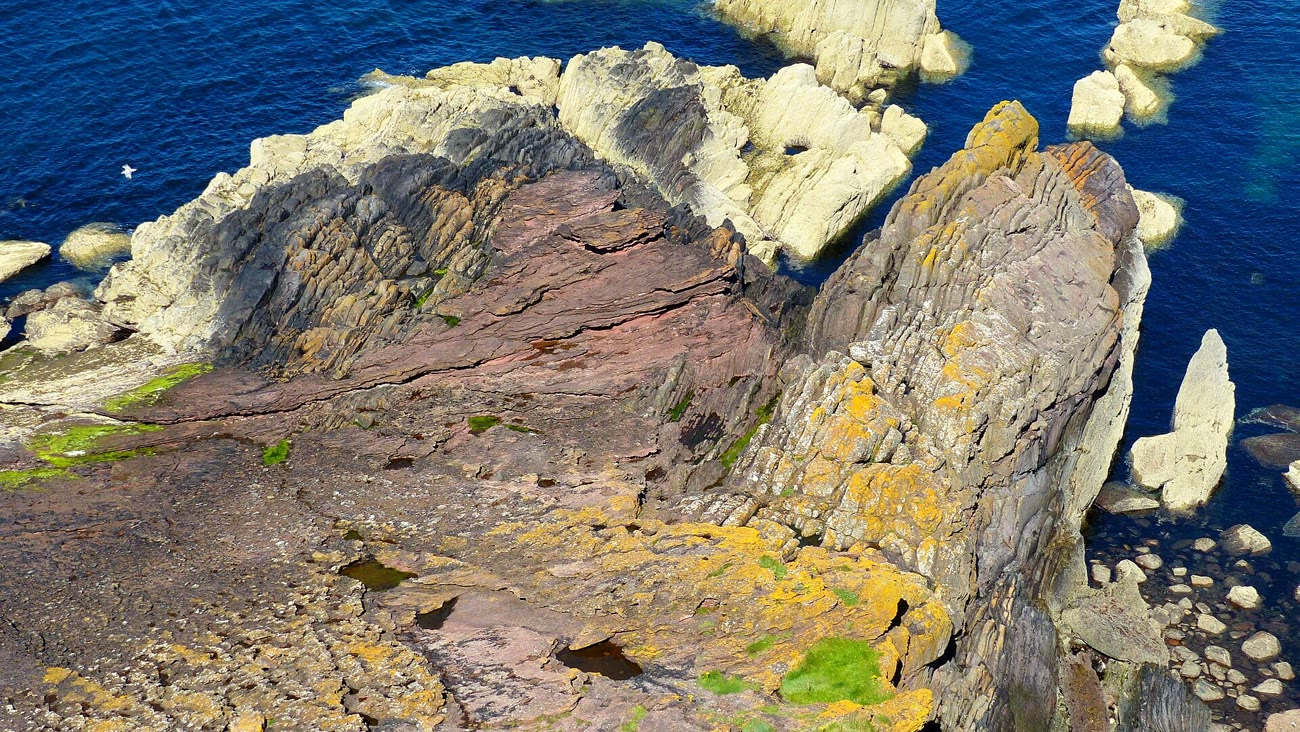
\includegraphics[width=0.7\linewidth]{images/book3/b1-siccar-point.jpg}

{\small \omterm{def:b1:cross-sections:unconformity}{Discordancia} de Hutton en Siccar Point: capas grises silúricas casi verticales debajo,
capas rojas devónicas suavemente inclinadas encima. Fotografía PawełS, CC BY-SA 4.0 (Wikimedia
Commons).}
% ledger: commons:siccar-point
\end{center}
\end{history}

\begin{inthefield}[Geología para un túnel]
\begin{minipage}[t]{0.6\linewidth}\vspace{0pt}
Antes de diseñar un túnel, los geólogos de ingeniería construyen cortes a lo largo de su línea a
partir del \omterm{def:b1:geological-maps:geological-map}{mapa geológico}, de sondeos perforados a intervalos a lo largo del trazado y de
prospecciones geofísicas. Predicen cada unidad que cortará el túnel, las fallas que cruzará y los
puntos donde puede entrar agua. Durante la excavación, los geólogos del contratista registran la roca
que queda al descubierto en el frente en cada avance, la comparan con la predicción y actualizan el
corte; los sondeos de reconocimiento que se perforan por delante de la máquina ponen a prueba el
terreno antes de que llegue a él, sobre todo cerca de una falla prevista o en la caliza, que puede
contener cavidades. Una zona de falla de roca triturada es un peligro clásico, tanto más cuando la
misma roca aparece a ambos lados y nada en el frente lo anuncia.
\end{minipage}\hfill
\begin{minipage}[t]{0.37\linewidth}\vspace{0pt}
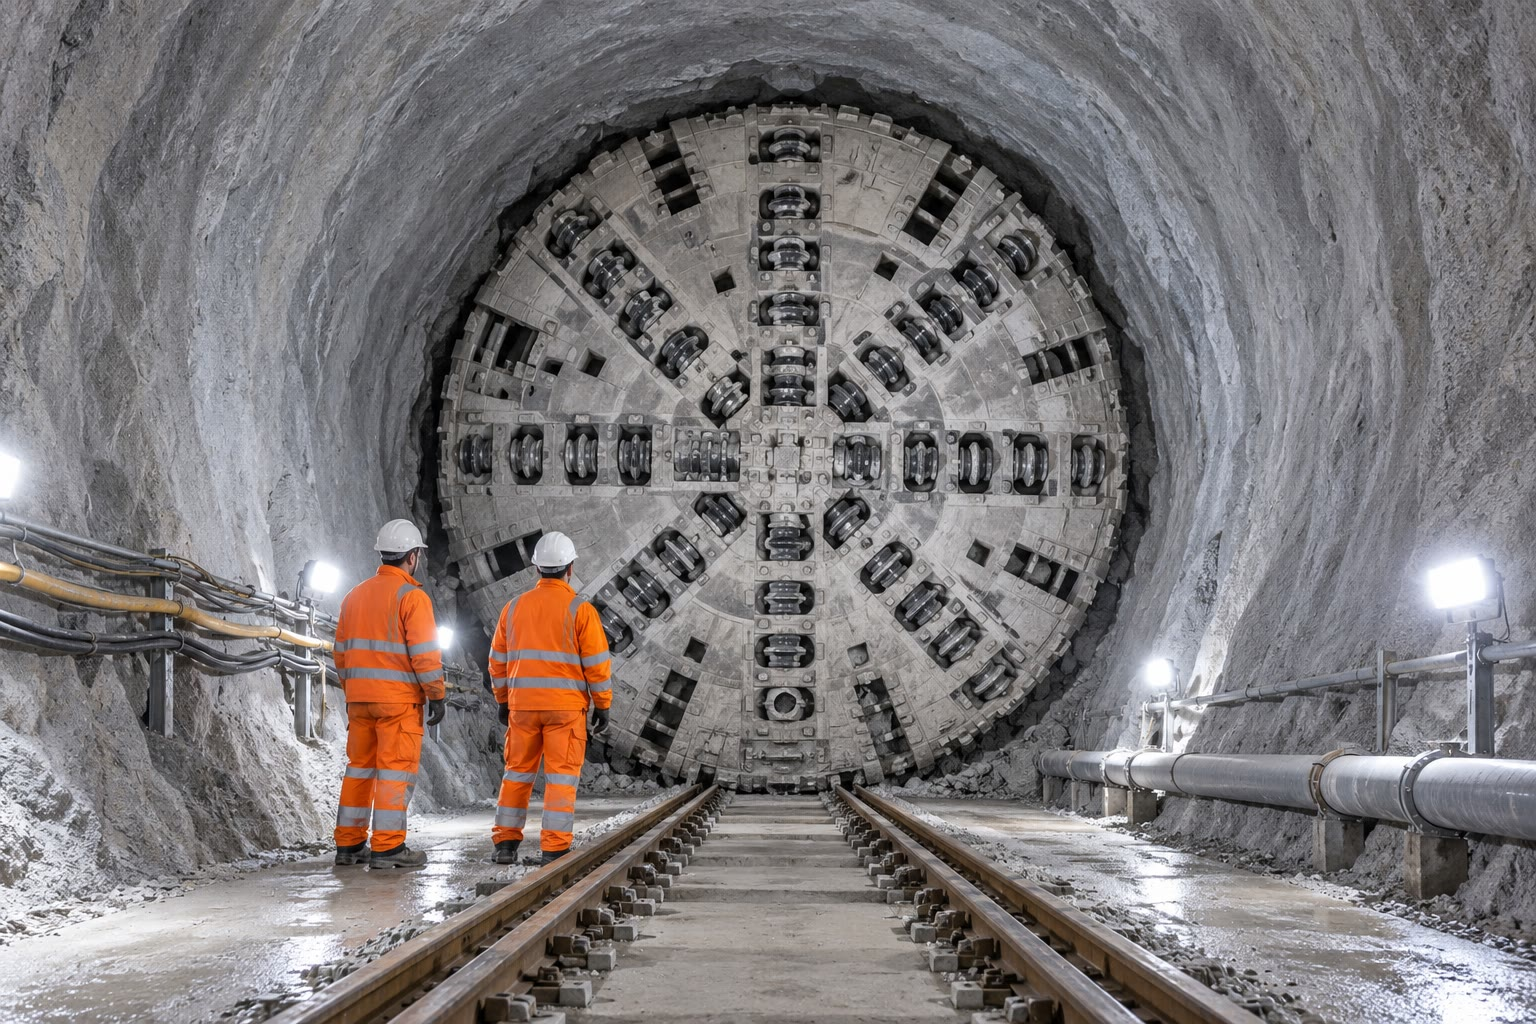
\includegraphics[width=\linewidth]{images/book3/ai/b1-tunnel-boring.jpg}
\end{minipage}
\end{inthefield}

\section{Ejercicios}

\begin{exercise}[$\star$]\label{exo:b1:cross-sections:1}
A partir de un mapa a escala 1:25\,000 se dibuja un corte con una escala vertical de \qty{1}{cm} por
cada \qty{100}{m}. ¿Cuál es su \omterm{def:b1:cross-sections:section}{exageración vertical}?
\end{exercise}

\begin{exercise}[$\star$]\label{exo:b1:cross-sections:2}
Un estrato buza \ang{40} hacia \ang{090}. ¿Cuál es su \omterm{def:b1:cross-sections:apparent-dip}{buzamiento aparente} en un corte vertical de
\omterm{def:b1:spherical-astronomy:horizontal}{acimut} \ang{060}? ¿Y en uno de \omterm{def:b1:spherical-astronomy:horizontal}{acimut} \ang{000}?
\end{exercise}

\begin{exercise}[$\star$]\label{exo:b1:cross-sections:3}
Un sondeo vertical atraviesa \qty{120}{m} de arenisca cuyos estratos buzan \ang{12.16}. ¿Cuál es el
\omterm{def:b1:cross-sections:thickness}{espesor verdadero} de la arenisca?
\end{exercise}

\begin{exercise}[$\star$]\label{exo:b1:cross-sections:4}
Un contacto que buza \ang{12} en el plano de un corte se dibuja con \omterm{def:b1:cross-sections:section}{exageraciones verticales} de 2, 3
y 5. ¿A qué ángulos aparece?
\end{exercise}

\begin{exercise}[$\star\star$]\label{exo:b1:cross-sections:5}
Una capa buza \ang{25}. Su afloramiento tiene \qty{300}{m} de anchura, medida perpendicularmente al
\omterm{def:b1:geological-maps:attitude}{rumbo}. Calcúlese su \omterm{def:b1:cross-sections:thickness}{espesor verdadero} (a) sobre terreno horizontal; (b) sobre un terreno con una
pendiente de \ang{10} en sentido contrario al \omterm{def:b1:geological-maps:attitude}{buzamiento}, siendo la anchura medida a lo largo del
terreno; (c) sobre un terreno con una pendiente de \ang{10} en el mismo sentido que el \omterm{def:b1:geological-maps:attitude}{buzamiento}.
\end{exercise}

\begin{exercise}[$\star\star$]\label{exo:b1:cross-sections:6}
Un estrato muestra un \omterm{def:b1:cross-sections:apparent-dip}{buzamiento aparente} de \ang{20} hacia el norte en un corte norte--sur, y de
\ang{30} hacia el este en un corte este--oeste. Hállense su \omterm{def:b1:geological-maps:attitude}{dirección de buzamiento} y su \omterm{def:b1:geological-maps:attitude}{buzamiento}
verdadero.
\end{exercise}

\begin{exercise}[$\star\star$]\label{exo:b1:cross-sections:7}
El muro de la caliza en el flanco oriental buza \ang{12.16}. ¿Cuál es la separación horizontal de
sus \omterm{def:b1:cross-sections:structure-contour}{curvas de nivel estructurales} trazadas cada \qty{100}{m}? Compruébese en el \omterm{def:b1:cross-sections:structure-contour}{mapa de curvas de
nivel estructurales}.
\end{exercise}

\begin{exercise}[$\star\star$]\label{exo:b1:cross-sections:8}
A partir de la tabla de sondeos, calcúlese la altitud de la base de la lutita en B1 y en B3. Sobre
B2 la lutita ha sido erosionada: a partir del \omterm{def:b1:cross-sections:thickness}{espesor vertical} de la caliza, hállese la altitud que
tendría su base allí, y el \omterm{def:b1:cross-sections:apparent-dip}{buzamiento aparente} de ese contacto entre B1 y B2 en el corte C--D.
¿Qué indica sobre el \omterm{def:b1:geological-maps:fold}{pliegue} la comparación de B1 y B3?
\end{exercise}

\begin{exercise}[$\star\star$]\label{exo:b1:cross-sections:9}
Una falla normal que buza \ang{50} hacia \ang{180} tiene un \omterm{def:b1:cross-sections:throw}{salto vertical} de \qty{150}{m}. Calcúlese
su \omterm{def:b1:cross-sections:throw}{salto horizontal}. En un corte vertical de \omterm{def:b1:spherical-astronomy:horizontal}{acimut} \ang{150}, ¿cuáles son el \omterm{def:b1:cross-sections:apparent-dip}{buzamiento aparente} de
la falla y la separación de los dos cortes de un estrato horizontal a lo largo del corte?
\end{exercise}

\begin{exercise}[$\star\star\star$]\label{exo:b1:cross-sections:10}
Para un estrato que buza \ang{40}, ¿en qué direcciones de corte el \omterm{def:b1:cross-sections:apparent-dip}{buzamiento aparente} es la mitad
del verdadero, es decir, \ang{20}? Demuéstrese que el \omterm{def:b1:cross-sections:apparent-dip}{buzamiento aparente} varía poco cerca de la
\omterm{def:b1:geological-maps:attitude}{dirección de buzamiento} y deprisa cerca del \omterm{def:b1:geological-maps:attitude}{rumbo}.
\end{exercise}

\begin{exercise}[$\star\star\star$]\label{exo:b1:cross-sections:11}
Un sondeo atraviesa la caliza del flanco oriental (\omterm{def:b1:cross-sections:thickness}{espesor verdadero} \qty{176.0}{m}, \omterm{def:b1:geological-maps:attitude}{buzamiento}
\ang{12.16} hacia \ang{080.7}). ¿Qué longitud de testigo recupera (a) si es vertical; (b) si está
inclinado \ang{60} bajo la horizontal hacia \ang{260.7}; (c) inclinado \ang{60} hacia \ang{080.7}?
(Pista: la longitud es $t/\cos\psi$, donde $\psi$ es el ángulo entre el sondeo y la normal a la
estratificación.)
\end{exercise}

\begin{exercise}[$\star\star\star$]\label{exo:b1:cross-sections:12}
En una \omterm{def:b1:cross-sections:unconformity}{discordancia angular}, los estratos inferiores buzan \ang{70} hacia \ang{090} y los superiores
\ang{20} hacia \ang{270}, con el mismo \omterm{def:b1:geological-maps:attitude}{rumbo}. Gírese todo el afloramiento alrededor del \omterm{def:b1:geological-maps:attitude}{rumbo} para
devolver a la horizontal los estratos superiores: ¿cuál era el \omterm{def:b1:geological-maps:attitude}{buzamiento} de los inferiores cuando se
depositaron los superiores? Escríbase en orden la historia del afloramiento.
\end{exercise}

\section{Problema: un túnel bajo las colinas de Varden}

\begin{problem}[{Problema de fin de semana --- qué rocas cortará un túnel, dónde encontrará la falla
y cuánta caliza perforará}]
\label{pb:b1:cross-sections:1}
% numbers from figdata/bachelor-1/varden_sections.py (model region.py) and the scratch calculator
El túnel discurre exactamente hacia el este a lo largo de la línea C--D ($y = \qty{6}{km}$), a la
altitud constante de \qty{200}{m}, desde $x = \qty{1}{km}$ hasta $x =
\qty{9}{km}$. La altitud del terreno a lo largo de C--D es, cada kilómetro
desde
$x = 0$:
\begin{center}
\small
\begin{tabular}{lccccccccccc}
\hline
$x$ (km) & 0 & 1 & 2 & 3 & 4 & 5 & 6 & 7 & 8 & 9 & 10 \\
$z$ (m) & 509 & 556 & 467 & 370 & 435 & 534 & 501 & 455 & 406 & 339 & 405 \\
\hline
\end{tabular}
\end{center}
Utilícense la tabla de sondeos del capítulo, el corte C--D dibujado con $e = 3$, la \omterm{def:b1:geological-maps:attitude}{actitud} del
flanco oriental (\omterm{def:b1:geological-maps:attitude}{buzamiento} \ang{12.16} hacia \ang{080.7}; el flanco occidental es su imagen
especular, que buza hacia \ang{279.3}), y la falla normal, que buza \ang{60} hacia \ang{120}, tiene
un \omterm{def:b1:cross-sections:throw}{salto vertical} de \qty{200}{m} y pasa por el punto $x = \qty{4.30}{km}$, $y = \qty{1.00}{km}$,
$z = \qty{250}{m}$.

\medskip
\noindent\textbf{Parte I --- El perfil y las unidades.}
\begin{enumerate}
  \item ¿Cuáles son el mayor y el menor espesor de roca sobre el túnel en los puntos kilométricos
        entre $x = 1$ y $x = 9$?
  \item En el corte impreso, \qty{1}{km} de distancia horizontal mide \qty{1.4}{cm}, y \qty{1}{km}
        de altitud mide \qty{4.2}{cm}. Compruébese que $e = 3$.
  \item A partir del registro de B2, hállese la altitud de la base de la arenisca en la cresta del
        \omterm{def:b1:geological-maps:fold}{anticlinal}.
  \item ¿En qué unidad está el túnel en $x = \qty{3.5}{km}$?
  \item Calcúlese la altitud de la base de la caliza en B1 y en B3.
  \item A partir del corte, enumérense en orden las unidades que atraviesa el túnel desde $x = 1$
        hasta $x = \qty{9}{km}$.
\end{enumerate}

\medskip
\noindent\textbf{Parte II --- Buzamientos en el corte.}
\begin{enumerate}[resume]
  \item Calcúlese el \omterm{def:b1:cross-sections:apparent-dip}{buzamiento aparente} del flanco oriental en C--D a partir de su \omterm{def:b1:geological-maps:attitude}{actitud}.
  \item Compruébese a partir de las altitudes de la base de la caliza en B2 y en B3.
  \item ¿Con qué ángulo se dibuja el flanco oriental en el corte con $e = 3$?
  \item Calcúlese el \omterm{def:b1:cross-sections:apparent-dip}{buzamiento aparente} de la falla en C--D.
  \item ¿Por qué el \omterm{def:b1:cross-sections:apparent-dip}{buzamiento aparente} de los flancos en C--D está tan cerca de su \omterm{def:b1:geological-maps:attitude}{buzamiento}
        verdadero, y el de la falla, menos?
\end{enumerate}

\medskip
\noindent\textbf{Parte III --- La falla.}
\begin{enumerate}[resume]
  \item Muéstrese que, en el plano $y = \qty{6}{km}$, la falla está en
        \[ x = 4300 + \frac{2500 - (z - 250)\tan\ang{30}}{\sin\ang{120}}
           \quad\text{(metros)}. \]
  \item ¿Dónde encuentra el túnel a la falla?
  \item Calcúlese el \omterm{def:b1:cross-sections:throw}{salto horizontal} de la falla y la separación de los cortes de un contacto a lo
        largo de C--D.
  \item ¿Qué bloque está hundido, y qué unidad queda a la altura del túnel a cada lado de la falla?
  \item ¿Por qué es la falla un peligro que la cuadrilla no podía ver venir desde la roca del frente?
        ¿Cómo lo previenen los ingenieros?
\end{enumerate}

\medskip
\noindent\textbf{Parte IV --- La caliza.}
\begin{enumerate}[resume]
  \item ¿Cuál es el \omterm{def:b1:cross-sections:thickness}{espesor vertical} de la caliza en B1?
  \item ¿Cuál es su \omterm{def:b1:cross-sections:thickness}{espesor verdadero}?
  \item Muéstrese que, al oeste de la falla en C--D, la base de la arenisca está
        en
        \[ z_b = 160.16 - |x - 3500|\tan\ang{12.0} \quad\text{(metros)}. \]
  \item El túnel está en la caliza cuando su base queda por debajo de \qty{200}{m} y su techo por
        encima. Muéstrese que esto ocurre para $377.1 < |x - 3500|
        < 1224.0$.
  \item Dense los cuatro puntos donde el túnel entra en la caliza y sale de ella.
  \item Muéstrese que la longitud perforada en cada flanco es $h/\tan\beta$, donde $h$ es el
        \omterm{def:b1:cross-sections:thickness}{espesor vertical} y $\beta$ el \omterm{def:b1:cross-sections:apparent-dip}{buzamiento aparente}, y calcúlese.
  \item ¿Qué longitud total de caliza atraviesa el túnel?
\end{enumerate}
\end{problem}
